\chapter{AFABL: A Friendly Adaptive Behavior Language}\label{ch:afabl}

AFABL is an internal domain-specific language (DSL) shallowly embedded in the Scala programming language. In this chapter we explain why we chose to implement AFABL as a Scala-embedded DSL, present the basic elements of AFABL with examples, and report the results of a programmer study which confirm and quantify the usefulness of integrating reinforcement learning into a programming language.

\section{Why an embedded DSL?}

We chose to implement AFABL as a shallowly embedded domain-specific language because of the exploratory nature of this research. Our goal at this point is to confirm our expectation that integrating reinforcement learning is useful to programmers writing agents, to explore the nature of this integration, and to get qualitative feedback from programmers on their experience using a language that integrates reinforcement learning. Writing a full language with its own lexical and syntactic structure, internal representations, and and tools (interpreters, compilers, linkers, etc.) would distract from the core questions we are trying to answer. As we discuss in Section \ref{sec:conclusion-full-language}, creating a full independent language is a direction for future research which will be guided by the results we present here, for which an embedded DSL is sufficient.

\section{Why Scala?}

Hosting DSLs is a primary design goal of the Scala programming language. Scala is an expressive and concise language which already enables the expression of domain models with little syntactic baggage. By employing just a few Scala language features that are designed for writing expressive and convenient libraries, we can create a DSL that Scala programmers will find familiar and non-Scala programmers can use to encode adaptive agents. Indeed, the nature of Scala's syntax and language features is such that many Scala libraries that are not explicitly labeled as DSLs qualify as shallow embedded DSLs.


\section{AFABL Concepts}

AFABL is a language for encoding adaptive (intelligent) agents. Before we present the AFABL language, we review basic adaptive agent concepts that can be encoded in AFABL.

%% \subsection{Terminology}

%% \begin{itemize}

%% \item State. A state is a configuration of all objects and agents in a world. These configurations can include object locations and orientations, mental or emotional dispositions of agents, or indications of the occurrence of events (e.g., agent X just got shot).

%% \item Perception, or Percept. A subset of a world state that is perceived by an agent (or module).

%% \item Action. An action is a one-shot state manipulation that can be executed by an agent.  Sometimes called "primitives," actions acquire greater meaning when they are executed (possibly in sequences) by behavior modules to achieve a goal or satisfy a constraint.


%% \item World. Sometimes called an "environment," a world is a container for all the things an agent can perceive and act upon, and possibly hidden things.  Worlds are represented by states that specify the configuration of all the things in a world at a given point in time.

%% \item World Dynamics. The dynamics of a world specifies the state transitions that are made in response to the execution of actions.  World dynamics may be deterministic or stochastic.  Markov Decision Processes are often used to represent world dynamics.

%% \item Behavior Module. A behavior module is a self-contained agent component that recommends an action (response) for a given state perception (stimulus).  Anything that produces a policy (a mapping from states to actions and tasks) is a behavior module.  A behavior module is sometimes called a "subagent" in modular reinforcement learning.

%% \item Agent. An agent is an entity that acts under its own control, perceiving the state of its world and executing actions in response to these perceived states.

%% \item Intelligent Agent. An intelligent agent is an agent that chooses its actions to achieve goals or satisfy constraints.

%% \item Adaptive Agent. An adaptive agent is an intelligent agent that can automatically adapt its behaviors to different worlds (that is, choose different actions sequences to achieve goals in worlds with different dynamics), or adapt its behaviors at run-time to worlds in which the dynamics change.

%% \item Modular Agent. A modular agent is an agent that consists of multiple behavior modules and performs command arbitration to decide which module's preferred action to execute in a given state.

%% \item Command Arbitration. Command arbitration is the act of deciding, for a given state, which behavior module should choose the action for the agent.


%% \end{itemize}

\subsection{Agent Architecture}

An AFABL agent is a behavioral agent that is composed of reusable behavior modules.  By "behavioral agent" we mean that the agent executes an action in response to a stimulus, represented by a state observation.  Each behavior module is itself an agent that has a preferred action for each state.  AFABL agents perform command arbitration to choose one of the modules' recommended actions for each state.  The behavior modules recommend actions in each state, and the arbitrator chooses which module to "listen to" in each state.  The AFABL agent architecture is a subsumption architecture \cite{brooks1986a-robust}.

\subsection{Behavior Modules}

Behavior modules, sometimes called subagents in the modular reinforcement learning literature, are agents that are meant to be combined to form larger agents.  Behavior modules are similar to the layers of Brooks's subsumption architecture with an important difference: autonomy.  The internal working of a behavior module is never altered externally.  A behavior module defines a state abstraction that converts the state observation it is given to a (possibly) simpler state that is used internally for decision making and learning.  The decision making and adaptation mechanisms inside a module remain completely under the module's control.  Interaction with the module consists entirely of reporting a state observation to the module, asking the module for an action, and reporting to the module the effect of executing an action.

\subsection{Adaptive Modules}

An adaptive module employs learning algorithms under the hood to achieve automatic adaptivity.  By adaptive we mean two things: (1) adaptation to new worlds, and (2) run-time adaptation.  A module that is programmed to work for worlds with a given state representation will work with any world that provides the same state representation, even if the dynamics of the worlds differ.  An adaptive module need simply be retrained for the new world.  Once an adaptive module is running in an active agent, the module may continue to tune its internal learning models as the agent acts in the world, providing for run-time adaptation.

\subsection{Command Arbitrators}

Command arbitrators take as input the state of the world and possibly the action preferences of a set of modules, and selects one of the modules or actions to be executed by the agent.

\section{The AFABL Language}

AFABL is a framework/DSL in the Scala programming language for implementing adaptive agents. An AFABL agent operates in a world, is composed of one or more modules, and has an agent level reward function that it uses to learn a command arbitration policy.

\subsection{Worlds}

Every AFABL module and agent is designed to operate in a world. A world defines the states, actions and state transition dynamics for a given state and action types. Details are discussed below.

\subsubsection{States}

The states of a world can be represented with any kind of Scala class. Case classes (\ref{sec:scala-case-classes}) are good for representing states because of their concise syntax and built-in equality methods. Figure \ref{fig:bunny-state-code} shows a case class for a state with three state variables: the locations of a bunny, wolf, and food.

\begin{figure}[!h]
\begin{center}

\begin{lstlisting}[language=Scala]
case class Location(x: Int, y: Int)

case class BunnyState(
  bunny: Location,
  wolf: Location,
  food: Location
)
\end{lstlisting}

\caption{Scala code to represent states in the bunny world.}
\end{center}
\label{fig:bunny-state-code}
\end{figure}

\subsubsection{Actions}

Actions are represented by objects which can be instances of any class. As with states, case classes make a good choice for implementing actions. Figure \ref{fig:bunny-action-code} shows actions for the bunny world implemented as a Scala enumeration (\ref{sec:scala-enumerations}).

\begin{figure}[!h]
\begin{center}

\begin{lstlisting}[language=Scala]
object BunnyAction extends Enumeration {
  val Up = Value("^")
  val Down = Value("v")
  val Left = Value("<")
  val Right = Value(">")
}
\end{lstlisting}

\caption{Scala code to represent the actions that the bunny agent can take in the bunny world.}
\end{center}
\label{fig:bunny-action-code}
\end{figure}

\subsubsection{World Dynamics}

An agent executes actions in a world, and those actions potentially change the state of the world. Having defined Scala representations for states and actions, we can define a world. Figure \ref{fig:world-code} shows the abstract class which defines the basic interface of world objects, which are instances of subclasses if {\tt World}. As we discuss in Sections \ref{sec:afabl-modules} and \ref{sec:afabl-agents}, all modules and agents are defined to act in a particular instance of a world. As with states and actions, world representations make no advanced use of the Scala programming language.

\begin{figure}[!h]
\begin{center}
\small
\begin{lstlisting}[language=Scala]
abstract class World[S, A] {
  def init(): S
  def resetAgent(): S
  def states: Seq[S]
  def actions: Seq[A]
  def act(action: A): S
}
\end{lstlisting}
\normalsize
\caption{The abstract superclass of all world classes for AFABL agents.}
\end{center}
\label{fig:world-code}
\end{figure}

%% \begin{figure}[p]
%% \begin{center}
%% \small
%% \begin{lstlisting}[language=Scala]
%% /** A stateful object representing world dynamics.
%%   */
%% abstract class World[S, A] {

%%   /** Initialize the world to a start state.
%%     */
%%   def init(): S

%%   /** Move agent to a start state, according to the rules of the
%%     * implementing world. Useful for continuing worlds where there is
%%     * no terminal state and the agent "respawns" after dying.
%%     */
%%   def resetAgent(): S

%%   /** All the states of this world. Necessary for reinforcement learning
%%     * agents.
%%     */
%%   def states: Seq[S]

%%   /** All the actions an agent can execute in this world.  For
%%     * simplicity this includes all the actions, and the actions that
%%     * aren't available in a given state simply have no
%%     * effect. Necessary for reinforcement learning agents.
%%     */
%%   def actions: Seq[A]

%%   /** Execute action in the world, resulting in a (possibly) new state.
%%    */
%%   def act(action: A): S
%% }
%% \end{lstlisting}
%% \normalsize
%% \caption{The abstract superclass of all world classes for AFABL agents.}
%% \end{center}
%% \label{fig:world-code}
%% \end{figure}


Figure \ref{fig:bunny-world-code} shows some of the code for the Bunny World.

\begin{figure}[!h]
\begin{center}
\small
\begin{lstlisting}[language=Scala]
class BunnyWorld(val width: Int = 5, val height: Int = 5)
  extends World[BunnyState, BunnyAction.Value] with LazyLogging {

  // Initialize the world state
  var state = init()

  // In Scala, defs can be overridden with vals
  val states = {
    // Calculate every possible combination of locations for the
    // bunny, wolf, and food
  }

  // This line returns all the values of the BunnyAction enumeration
  val actions = BunnyAction.values.toSeq

  def init(): BunnyState = {
    // Calculate initial locations for the bunny, wolf, and food.
    //
  }

  def resetAgent(): BunnyState = {
    // "Respawn" the bunny at a new location, update the world state
    // and return the new state
  }

  def act(intendedAction: BunnyAction.Value): BunnyState = {
    // Code to calculate the actual action due to uncertainty in the
    // environment and update the state of the world based on the
    // actual action.
  }
  // Helper functions ...
}
\end{lstlisting}
\normalsize
\caption{Parts of the bunny world class showing important aspects of the implementation of the {\tt World} abstract class.}
\end{center}
\label{fig:bunny-world-code}
\end{figure}


\subsection{Modules}\label{sec:afabl-modules}

Figure \ref{fig:find-food-code} shows the complete code for an AFABL implementation of a behavior module that represents the goal of finding food. First is the definition of a case class, {\tt FindFoodState}, to represent the state abstraction for FindFood modules. {\tt FindFoodState} includes only two of the three state variables in the bunny world.

\begin{center}
\begin{lstlisting}[language=Scala,frame=none]
case class FindFoodState(bunny: Location, food: Location)
\end{lstlisting}
\end{center}

We store a reference to an {\tt AfablModule} for FindFood in {\tt findFood}.

\begin{center}
\begin{lstlisting}[language=Scala,frame=none]
val findFood = AfablModule(
\end{lstlisting}
\end{center}

The {\tt AfablModule} factory method takes three arguments: an instance of a {\tt World} that the module can act and learn in, a {\tt stateAbstraction} function, and a {\tt moduleReward} function.

The first argument to {\tt AfablModule} is the world:

\begin{center}
\begin{lstlisting}[language=Scala,frame=none]
world = new BunnyWorld
\end{lstlisting}
\end{center}

The {\tt world} and {\tt =} are optional, but if included must be verbatim, i.e., considered part of the AFABL language.

The second argument is a state abstraction function that takes a world-state object as a parameter and returns an instance of our state abstraction class:

\begin{center}
\begin{lstlisting}[language=Scala,frame=none]
stateAbstraction = (worldState: BunnyState) => {
  FindFoodState(worldState.bunny, worldState.food)
}
\end{lstlisting}
\end{center}

The {\tt stateAbstraction} and {\tt =} are optional, but if included should be considered part of the AFABL language. {\tt worldState} is a user-chosen name, {\tt BunnyState} must match the state type defined for the world in which the module and agent operate, in this case it is the first type parameter to {\tt World} in the {\tt BunnyWorld} code in Figure \ref{fig:bunny-world-code}. The last expression in the body of the {\tt stateAbstraction} function must be an instance of a module state, in this case {\tt FindFoodState}.

The third and final argument to the {\tt AfablModule} factory method is a module reward function that takes an instance of our state abstraction class and returns the reward this module receives for being in that state:

\begin{center}
\begin{lstlisting}[language=Scala,frame=none]
moduleReward = (moduleState: FindFoodState) => {
  if (moduleState.bunny == moduleState.food) 1.0
  else -0.1
}
\end{lstlisting}
\end{center}

The {\tt moduleReward} and {\tt =} are optional, but if included should be considered part of the AFABL language. {\tt moduleState} is a user-chosen name, but the parameter type, {\tt FindFoodState} in this example, must match the return type of the {\tt stateAbstraction} function. The last expression in the body of the {\tt moduleReward} function must be a {\tt Double} value. In this case, which is typical, the body of the {\tt moduleReward} function is an {\tt if} expression which simply returns the reward based on state predicates. This example is another case where we could have implemented DSL-specific syntax, such as a list of predicates and values, but the syntactic overhead of Scala's {\tt if} expression is minimal and the code is crystal clear to any Scala programmer.

These three components -- world, state abstraction and module reward -- define a module specific learning problem on a subset of the world in which the module (and agent containing the module) may act. Internally, AFABL uses these components to instantiate a Sarsa learning algorithm using the algorithm parameters discussed in Chapter \ref{ch:arbiq}, but the programmer need not be aware of any details of reinforcement learning {\it algorithms}. The AFABL programmer need only be familiar with the reinforcement learning {\it problem}.

\begin{figure}[!h]
\begin{center}

\begin{lstlisting}[language=Scala]
case class FindFoodState(bunny: Location, food: Location)

val findFood = AfablModule(
  world = new BunnyWorld,

  stateAbstraction = (worldState: BunnyState) => {
    FindFoodState(worldState.bunny, worldState.food)
  },

  moduleReward = (moduleState: FindFoodState) => {
    if (moduleState.bunny == moduleState.food) 1.0
    else -0.1
  }
)
\end{lstlisting}

\caption{AFABL code for a module that represents the goal of constantly finding food.}
\end{center}
\label{fig:find-food-code}
\end{figure}

This module example shows the value of splitting the world dynamics from the agent module's reward function. We can think of the world and the agent independently. In essence, the definition of a full MDP is split across the definition of a world, and the definition of an agent that acts in that world.

Here we also begin to see syntactic conveniences afforded by the AFABL DSL. There are only two type annotations and one control structure (in the reward function). The rest of the types are inferred by Scala's type inferencer thanks to the way we wrote the factory method that creates {\tt AfablModule}s. It's worth noting that we could have refined the DSL to further strip the few Scala syntactic artifacts (like the {\tt if} statement and the anonymous functions for {\tt stateAbstraction} and {\tt moduleReward}) but the syntactic overhead is minimal and there is a tradeoff between writing specific DSL syntax and using Scala's built-in syntax directly. Creating unique syntax for a DSL imposes cognitive burden on programmers who are proficient in the host language. The benefit of the unique syntax must outweigh this cognitive burden. Here we hope to strike the right balance between convenient domain-specific syntax and familiarity to programmers. Thanks to Scala's already concise and expressive language and idioms, although this looks like a DSL there is no special syntax in this example. This code is a good example of shallow DSL embedding.

\subsection{Agents}\label{sec:afabl-agents}

An AFABL agent is an agent that acts in a particular world, is composed of independent behavior modules pursuing their own continuing goals, and has a central command arbitrator that uses an agent level reward function to learn when it should listen to each module. As the code in Figure \ref{fig:afabl-bunny-code} shows, an AFABL agent allows programmers to express these components concisely, with very little cognitive distance between the concepts that make up the agent and the code that represents them. As with modules, {\tt AfablAgent} uses features of the Scala programming language to make the syntax more convenient. For example, there is only one explicit type annotation in the AFABL bunny agent code in Figure \ref{fig:afabl-bunny-code}, but behind the scenes a carefully written factory method in the companion object allows Scala's static type inferencer to infer type parameters of the {\tt AfablAgent} constructor, return types for anonymous functions, and assign a concrete type value to a path-dependent abstract type variable. Figuring out all this stuff and wrestling with Scala's type checker directly is not easy. Writing an AFABL agent is easy.

\begin{figure}[!h]
\begin{center}

\begin{lstlisting}[language=Scala]
val bunny = AfablAgent(
  world = new BunnyWorld,

  modules = Seq(findFood, avoidWolf),

  agentLevelReward = (state: BunnyState) => {
    if (state.bunny == state.wolf) 0.0
    else if (state.bunny == state.food) 1.0
    else 0.5
  }
)
\end{lstlisting}

\caption{An AFABL agent that acts in a world, contains behavior modules, and has an agent level reward.}
\end{center}
\label{fig:afabl-bunny-code}
\end{figure}



\subsection{A Complete AFABL Bunny}

A complete bunny agent using the AFABL DSL is shown in Figure \ref{fig:afabl-bunny-code}. This code would typically fit in a single editor window and represents a tremendous amount of functionality. This agent pursues two goals simultaneously and prioritizes them based on the relative locations of the bunny, the food, and the wolf.

\begin{figure}[!h]
\begin{center}

\begin{lstlisting}[language=Scala]
val bunnyWorld = new BunnyWorld

case class FindFoodState(bunny: Location, food: Location)
val findFood = AfablModule(
  world = bunnyWorld,
  stateAbstraction = (worldState: BunnyState) => {
    FindFoodState(worldState.bunny, worldState.food)
  },
  moduleReward = (moduleState: FindFoodState) => {
    if (moduleState.bunny == moduleState.food) 1.0
    else -0.1
  }
)

case class AvoidWolfState(bunny: Location, wolf: Location)
val avoidWolf = AfablModule(
  world = bunnyWorld,
  stateAbstraction = (worldState: BunnyState) => {
    AvoidWolfState(worldState.bunny, worldState.wolf)
  },
  moduleReward = (moduleState: AvoidWolfState) => {
    if (moduleState.bunny == moduleState.wolf) -0.1
    else 0.1
  }
)

val bunny = AfablAgent(
  world = new BunnyWorld,
  modules = Seq(findFood, avoidWolf),
  agentLevelReward = (state: BunnyState) => {
    if (state.bunny == state.wolf) 0.0
    else if (state.bunny == state.food) 1.0
    else 0.5
  }
)
\end{lstlisting}

\caption{A complete bunny agent in the AFABL DSL. Code for the modules is repeated from previous figures to give a sense of the full quantity of code required to write an agent with two behavior modules.}
\end{center}
\label{fig:afabl-bunny-code}
\end{figure}


\section{Experiments}

AFABL supports a declarative style in which the agent programmer specifies which states are desirable and undesirable, but not how the agent should choose actions to pursue or avoid those states. Action selection logic is derived automatically by reinforcement learning algorithms that the AFABL programmer never sees. AFABL also provides agent-based software abstractions that permit code to be reused in new domains. This reuse is one of the things we mean by adaptivity: existing AFABL code can adapt to new domains without modifying the code. We quantify the value of AFABL's agent programming abstractions in the experiments discussed below.

Programmers were randomly assigned to two equally-sized groups based on their demographics (see Appendix \ref{ch:programmer-study} for details): one group used Scala without AFABL first -- the Scala-first group -- and the other group used AFABL first -- the AFABL-first group.  Each group completed two programming tasks using Scala and AFABL in the order determined by their group.  For each task the programmers were asked to write elegant code that meets the requirements of the task as quickly as possible, balancing the quality of their solutions with time.  The idea was to get a good solution quickly, not a perfect solution in a long time.

\subsection{Task 1: Bunny-Food-Wolf}\label{sec:task1}

\begin{figure}[h]

\begin{center}
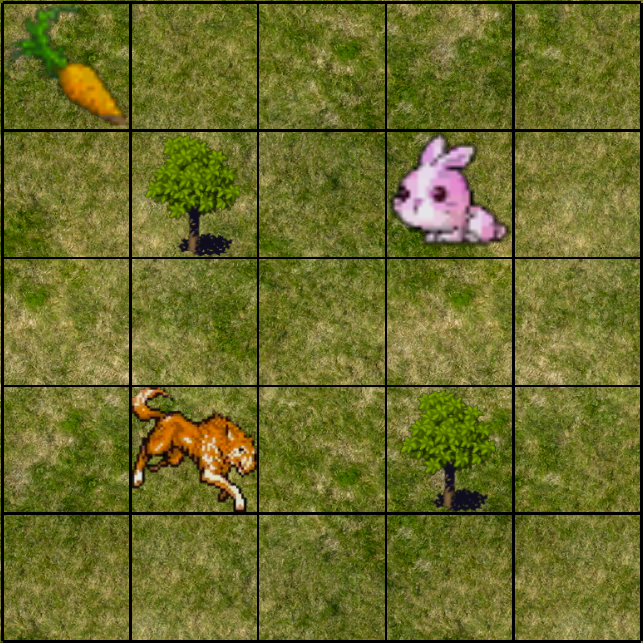
\includegraphics[height=2.4in]{bunny.png}
\end{center}


\caption{In the grid world above, the bunny must pursue two goals simultaneously: find food and avoid the wolf.  The bunny may move up, down, left, or right.  When it finds food it consumes the food and new food appears elsewhere in the grid world, when it meets the wolf it is eaten and ``respawns'' elsewhere.}
\label{fig:bunny-picture}
\end{figure}

In this task each programmer wrote an agents that control a bunny character in a simple world, depicted in Figure~\ref{fig:bunny-picture}.  The bunny world works as follows:

\begin{itemize}

\item The bunny world is a discrete grid of cells.  The bunny, wolf, and food each occupy one cell.

\item During each time step the bunny may move north, south, east, or west -- this is the bunny agent's action set.

\item Every two time steps the wolf moves towards the bunny.

\item If the bunny moves to the cell currently occupied by the food, the agent should be written to recognize this fact and give the agent an appropriate reward signal. In any case the simulation assumes food is ``eaten'' and new food appears elsewhere.

\item If the wolf moves to the cell currently occupied by the bunny it eats the bunny and the bunny ``respawns'' in a new location.

\end{itemize}

Programmers were asked to write bunny agents that meet the wolf as little as possible and eat as much food as possible.

\subsection{Task 2: Mating Bunny}\label{sec:task2}

In this task each programmer wrote a bunny agent for a world that is identical to the world in Task 1 except that the bunny must also find mates.  This world includes one static  potential mate that behaves similarly to the food.  When the bunny finds the potential mate, the simulation assumes that the bunny has ``mated,'' the mate disappears, and another potential mate appears elsewhere.  The simulation runs as in Task 1, and the scorer additionally keeps track of how many mates the bunny finds.  As in Task 1, programmers were asked to write bunny agents that meet the wolf as little as possible, eat as much food as possible, and find as many mates as possible.

%% \subsection{Task 3: Adding Wind, Spoiling Food, and Picky Mates}\label{sec:task3}

%% In this task each programmer will write a bunny agent for a world with the same elements as in Task 2 and with the same goals for the bunny, but the world is more complex.  In particular:

%% \begin{itemize}

%% \item There is constant wind from an unchanging direction that affects the wolf's ability to find the bunny.  The wolf will only move toward the bunny if the wolf is downwind of the bunny.

%% \item If food is not eaten within 15 time steps after it appears, it spoils.  Spoilage is represented by the food disappearing and new food appearing elsewhere.

%% \item To simulate selection of fit bunnies, potential mates will only accept the bunny if the bunny has eaten within 10 time steps (a hungry bunny is an unsuccessful bunny and therefore not fit for mating).  Rejection will be represented by the potential mate remaining in place and the bunny not receiving a signal that mating has occurred.

%% \end{itemize}

\subsection{Provided Code}

Study participants were given starter code so they could focus on writing the behavior of their agents. We provided the world for each task and the files in which to write their code. Participants were also given general documentation for AFABL but assumed to already be proficient in Scala.

Figure \ref{fig:scala-task1-provided} shows the code given to participants for the Scala bunny on Task 1. Figure \ref{fig:afabl-task1-provided} shows the code given to participants for the AFABL bunny on Task 1. The {\tt BunnyWorld}, {\tt BunnyState}, and {\tt BunnyAction} classes were also provided. It was up to participants to write state abstraction classes if they chose to do so.


\begin{figure}[!h]
\begin{center}

\begin{lstlisting}[language=Scala]
class ScalaBunny1 extends Agent[BunnyState, BunnyAction.Value]
    with Task1Scorer {

  // Your code goes in the body of this method. This method defines
  // your agent's behavior, that is, what action it takes in a given
  // state. The last expression in this method must be a
  // BunnyAction.  You may create as many helper functions as you
  // like, but please do not alter any of the provided code.
  def getAction(state: BunnyState, shouldExplore: Boolean = false) = {

    // This is a stub to make the code compile. Please
    // replace this with your code.
    BunnyAction.Up
  }
}
\end{lstlisting}

\caption{Starter Scala code provided to participants for Task 1.}
\end{center}
\label{fig:scala-task1-provided}
\end{figure}


\begin{figure}[!h]
\begin{center}

\begin{lstlisting}[language=Scala]
object AfablTask1 {

  // Use this val in your agent definitions.
  val bunnyWorld = new BunnyWorld

  // Please place all of your AFABL code for Task 1 in this singleton
  // object.


  // Your solution must assign your AFABL bunny agent for Task 1 to
  // the val afablBuny1.
  val afablBunny1 = ???
}
\end{lstlisting}

\caption{Starter AFABL code provided to participants for Task 1.}
\end{center}
\label{fig:afabl-task1-provided}
\end{figure}


The provided code for Task 2 was identical to the provided code for Task 1, except for the names of the files. For Task 2 participants were encouraged to copy code from Task 1 if they found it helpful, or to use any objects defined for Task 1 that would be helpful, such as behavior modules. As we discuss below, reusing code was straightforward for the AFABL agents but not for the Scala agents. As in Task 1, it was up to participants to write state abstraction classes if they chose to do so, but they could reuse any state abstraction classes written for Task 1.

Each task had a main method which ran the agents in the world to evaluate their performance.

\section{Quantitative Results}

We analyzed the submissions of study participants to compare Scala agents to AFABL agents in terms of code size, time spent writing Scala versus AFABL agents, the complexity of Scala versus AFABL agent code, and the performance of the agents on the assigned tasks.

\subsection{Code Size}

The size of a code base is often correlated with the level of effort required to write or understand the code. We computed the number of lines of code for each agent, not including comments.

\subsection{Time}

Study participants used the IntelliJ IDEA IDE with a plug-in that we wrote especially for this study. The plug-in recorded timestamps each time the editor tab with Task 1 or Task 2 files gained or lost the focus. We processed these logs to add up the time deltas between gaining and losing focus as an indication of the time programmers spent writing the code for each bunny agent.

\subsection{Cyclomatic Complexity}

We computed a complexity measure for all the submitted bunny agents. For Scala code we employed the simplified McCabe cyclomatic complexity measure \cite{mccabe1976complexity}:

\begin{equation}
v = \pi + 1
\end{equation}

where $v$ is the complexity score and $\pi$ is the number of predicates in decision structures.

\subsection{Performance}

Each programmer's Scala bunny and AFABL bunny were run for 1000 time steps and their average scores recorded. The score is based on how much food the bunny eats and how many times the bunny is eaten by the wolf for Task 1, and additionally how many times the bunny mates for Task 2. The score is normalized by the number of steps to indicate a sort of ``happiness index,'' a ratio of rewards to lifespan. This score happens to correspond to the measure used to validate Arbi-Q in Chapter \ref{ch:arbiq} to facilitate comparison between programmer authored agents and the performance of the algorithms we implemented for our reformulated MRL. It is important to note, however, that our aim here is not to achieve optimal performance but to create a programming system that makes it easy to write agents that achieve good performance.

\subsection{Typical Task 1 Submissions}

\begin{figure}[!h]
\begin{center}

\begin{lstlisting}[language=Scala]
class ScalaBunny1 extends Agent[BunnyState, BunnyAction.Value]
    with Task1Scorer {

  def getAction(state: BunnyState, shouldExplore: Boolean = false) = {
    if (wolfNearFood(state))
      moveAwayFromWolf(state)
    else
      moveTowardFood(state)
   }

  def wolfNearFood(state: BunnyState) = {
    val wolfToFood = sqrt(pow(state.food.x - state.wolf.x, 2) +
                          pow(state.food.y - state.wolf.y, 2))
    val bunnyToFood = sqrt(pow(state.food.x - state.bunny.x, 2) +
                           pow(state.food.y - state.bunny.y, 2))
    wolfToFood < bunnyToFood
  }

  def moveTowardFood(state: BunnyState) = {
    if (state.food.x > state.bunny.x)
      BunnyAction.Right
    else if (state.food.x < state.bunny.x)
      BunnyAction.Left
    else if (state.food.y < state.bunny.y)
      BunnyAction.Up
    else
      BunnyAction.Down
  }

  def moveAwayFromWolf(state: BunnyState) = {
    if (state.wolf.x < state.bunny.x)
      BunnyAction.Right
    else if (state.wolf.x > state.bunny.x)
      BunnyAction.Left
    else if (state.wolf.y > state.bunny.y)
      BunnyAction.Up
    else
      BunnyAction.Down
  }
}
\end{lstlisting}

\caption{Typical Scala submission for Task 1.}
\end{center}
\label{fig:scala-task1-submission}
\end{figure}

Figure \ref{fig:scala-task1-submission} shows a typical Scala submission for Task 1. The action selection strategy is about as simple as possible. For example, there is no determination of where the wolf is in relation to the bunny and food other than distance. If the wolf is closer to the food than the bunny, move away from the wolf, otherwise move toward to the food. The agent does not distinguish between cases where the wolf is between the wolf and the food, or if the wolf is closer but sufficiently far away. One could imagine writing code to calculate the projection of the wolf's position onto the line between the bunny and the food to determine a safe closure rate for the wolf. However, this simple strategy is all that is needed to achieve nearly optimal results. This Scala-only bunny agent achieves an average performance score of 0.54, the same as the AFABL bunny.

\begin{figure}[!h]
\begin{center}

\begin{lstlisting}[language=Scala]
  case class FindFoodState(bunny: Location, food: Location)
  val findFood = AfablModule(
    world = bunnyWorld,
    stateAbstraction = (worldState: BunnyState) => {
      FindFoodState(worldState.bunny, worldState.food)
    },
    moduleReward = (moduleState: FindFoodState) => {
      if (moduleState.bunny == moduleState.food) 1.0
      else -0.1
    }
  )

  case class AvoidWolfState(bunny: Location, wolf: Location)
  val avoidWolf = AfablModule(
    world = bunnyWorld,
    stateAbstraction = (worldState: BunnyState) => {
      AvoidWolfState(worldState.bunny, worldState.wolf)
    },
    moduleReward = (moduleState: AvoidWolfState) => {
      if (moduleState.bunny == moduleState.wolf) -0.1
      else 0.1
    }
  )

  val afablBunny1 = AfablAgent(

    world = bunnyWorld,

    modules = Seq(findFood, avoidWolf),

    agentLevelReward = (state: BunnyState) => {
      if (state.bunny == state.wolf) 0.0
      else if (state.bunny == state.food) 1.0
      else 0.5
    }
  )
\end{lstlisting}

\caption{Typical AFABL submission for Task 1.}
\end{center}
\label{fig:afabl-task1-submission}
\end{figure}

Figure \ref{fig:afabl-task1-submission} shows a typical AFABL submission for Task 1. As in our earlier examples, the AFABL bunny is composed of behavior modules for finding food and avoiding the wolf. The AFABL documentation contained tips for reward authoring in modules and at the agent level.


The AFABL solution to Task 1 contains 31 lines of code and has a cyclomatic complexity of 5 (4 predicates in decision structures). The Scala solution to Task 1 uses 34 lines of code and has a cyclomatic complexity of 8 (7 predicates in decision structures). Both programs achieve the same nearly optimal level of performance with scores of ~0.54.

\subsection{Typical Task 2 Submissions}

\begin{figure}[!h]
\begin{center}

\begin{lstlisting}[language=Scala]
class ScalaBunny2 extends Agent[BunnyState, BunnyAction.Value]
    with Task2Scorer {

  def getAction(state: BunnyState, shouldExplore: Boolean = false) = {

    if ((distance(state.wolf, state.food) < distance(state.food, state.bunny))
      || distance(state.wolf, state.mate) < distance(state.mate, state.bunny))
      moveAwayFromWolf(state)
    else if (distance(state.bunny, state.food) < distance(state.bunny, state.mate))
      moveToward(state.bunny, state.food)
    else
      moveToward(state.bunny, state.mate)
  }

  def distance(a: Location, b: Location) = {
    sqrt(pow(a.x - b.x, 2) + pow(a.y - b.y, 2))
  }

  def moveToward(from: Location, to: Location) = {
    if (to.x > from.x)
      BunnyAction.Right
    else if (to.x < from.x)
      BunnyAction.Left
    else if (to.y > from.y)
      BunnyAction.Up
    else
      BunnyAction.Down
  }

  def moveAwayFromWolf(state: BunnyState) = {
    if (state.wolf.x < state.bunny.x)
      BunnyAction.Right
    else if (state.wolf.x > state.bunny.x)
      BunnyAction.Left
    else if (state.wolf.y > state.bunny.y)
      BunnyAction.Up
    else
      BunnyAction.Down
  }
}
\end{lstlisting}

\caption{Typical Scala submission for Task 2.}
\end{center}
\label{fig:scala-task2-submission}
\end{figure}

Figure \ref{fig:scala-task2-submission} shows a typical Scala solution for Task 2. While the Scala solution to Task 2 is more complex than the Scala solution to Task 1, it uses only one more line of code -- 35 -- due to refactoring of common logic. Of course, this refactoring took extra time and without the refactoring the line count and likely the cyclomatic complexity would have been higher.

\begin{figure}[!h]
\begin{center}

\begin{lstlisting}[language=Scala]
  case class FindMateState(bunny: Location, mate: Location)
  val findMate = AfablModule(
    world = bunnyWorld,
    stateAbstraction = (state: BunnyState) => {
      FindMateState(state.bunny, state.mate)
    },
    moduleReward = (state: FindMateState) => {
      if (state.bunny == state.mate) 1.0
      else -0.1
    }
  )

  // Your solution must assign your AFABL bunny agent for Task 2 to
  // the val afablBuny2.
  val afablBunny2 = AfablAgent(

    world = bunnyWorld,

    modules = Seq(AfablTask1.findFood, AfablTask1.avoidWolf, findMate),

    agentLevelReward = (state: BunnyState) => {
      if (state.bunny == state.wolf) 0.0
      else if (state.bunny == state.food) 1.0
      else if (state.bunny == state.mate) 1.0
      else 0.5
    }
  )
\end{lstlisting}

\caption{Typical AFABL submission for Task 2.}
\end{center}
\label{fig:afabl-task2-submission}
\end{figure}

Figure \ref{fig:afabl-task2-submission} shows typical AFABL code for Task 2. Notice that the {\tt findFood} and {\tt avoidWolf} modules from Task 1 have been reused directly. This works because the world, {\tt BunnyWorld}, is the same. In Task 1 the bunny was ignoring the mate. In Task 2 we adapt the bunny to find the mate, and all we need to do is add a {\tt findMate} module and add a line to the {\tt agentLevelReward} function so that the agent will also value finding mates.

The AFABL solution to Task 2 contains 21 lines of code due to reuse of modules from Task 1, and has the same cyclomatic complexity of 5 (4 predicates in decision structures) even though the agent is solving a more complex problem. Even with the refactoring of common logic in Task 2 the Scala solution has a higher cyclomatic complexity of 10 (9 predicates in decision structures), which McCabe says is the maximum allowable cyclomatic complexity for a testable, maintainable software module \cite{mccabe1976complexity}. Finally, the performance of the Scala solution to Task 2 decreases to 0.48, while the AFABL solution continues to achieve the same nearly optimal 0.54. With additional work perhaps the Scala agent's performance on Task 2 could have been improved, but the point here is that AFABL agents are easier to write, easier to adapt to new domains, have less complex code, and perform well without requiring a great deal of effort beyond choosing reward signals.

\subsection{Summary}

TBD ...

Quantitative results for Task 1 are summarized in Table \ref{tbl:task1-results}. Quantitative results for Task 2 are summarized in Table \ref{tbl:task2-results}.

\begin{center}
\begin{table}[h]
\begin{tabular}{|l|r|r|r|}\hline
                      & Scala Mean & AFABL Mean & p-value \\\hline
Lines of Code         & 0.0        & 0.0        & 0.0 \\
Time                  & 0.0        & 0.0        & 0.0 \\
Cyclomatic complexity & 0.0        & 0.0        & 0.0 \\
Performance           & 0.0        & 0.0        & 0.0 \\\hline
\end{tabular}
\caption{Quantitative results of Scala agent code versus AFABL agent code on Task 1. A p-value of less than .05 mean that the difference in means is statistically significant at the 95\% significance level, i.e. we reject $H_0: \mu_1 = \mu_2$ and conclude that the means are different.}
\label{tbl:task1-results}
\end{table}
\end{center}

\begin{center}
\begin{table}[h]
\begin{tabular}{|l|r|r|r|}\hline
                      & Scala Mean & AFABL Mean & p-value \\\hline
Lines of Code         & 0.0        & 0.0        & 0.0 \\
Time                  & 0.0        & 0.0        & 0.0 \\
Cyclomatic complexity & 0.0        & 0.0        & 0.0 \\
Performance           & 0.0        & 0.0        & 0.0 \\\hline
\end{tabular}
\caption{Quantitative results of Scala agent code versus AFABL agent code on Task 2. A p-value of less than .05 mean that the difference in means is statistically significant at the 95\% significance level, i.e., we reject $H_0: \mu_1 = \mu_2$ and conclude that the means are different.}
\label{tbl:task2-results}
\end{table}
\end{center}

\section{Qualitative Results}

TBD ...

Programmers responded to a questionnaire to give their impressions of agent programming in AFABL versus agent programming in Scala.

\begin{enumerate}
\item I have a positive impression of agent programming in Scala.

Rationale: programmers’ impression of Scala will provide a baseline for evaluating
programmers’ impression of AFABL.

\item I found it easier to write the agents using AFABL’s programming constructs compared to bare Scala.

Rationale: the point of AFABL is to facilitate agent programming, so programmers should have a more positive impression of AFABL for agent programming.

\item I believe that AFABL facilitated more reusable and maintainable code for agents compared to bare Scala.

Rationale: answers to this question should correlate with answers to Question 1.

\item If given the choice, I would choose AFABL over Scala for agent programming projects.

Rationale: answers to this question should correlate with answers to Question 2.

\item I found it easier to use AFABL compared to Scala for Task 1.

  Rationale: in addition to objective analyses of task submissions, we want to know whether programmers subjectively prefer AFABL.

\item What was it about AFABL that made the Task 1 easier or harder?

Rationale: we want to get open-ended feedback for things we did not anticipate.

\item I found it easier to use AFABL compared to Scala for Task 2.

Rationale: in addition to objective analyses of task submissions, we want to know whether programmers subjectively prefer AFABL.

\item What was it about AFABL that made the Task 2 easier or harder?

\end{enumerate}

\section{Conclusion}

As you can see from the similarity of the submission in Figure \ref{fig:afabl-task1-submission} to our explanatory example, most AFABL bunny agents look the same. There is one obvious way to implement a bunny agent that must pursue multiple goals. This uniformity is desirable. As Tim Peters says in the Zen of Python \cite{peters2004zen}, ``There should be one-- and preferably only one --obvious way to do it.'' The similarity in most AFABL solutions to a particular modular agent programming problem is an indication that AFABL provides the right abstractions for adaptive agent programming.
